\begin{figure}[h]
    \centering
    \begin{subfigure}{0.63\textwidth}
        \centering
        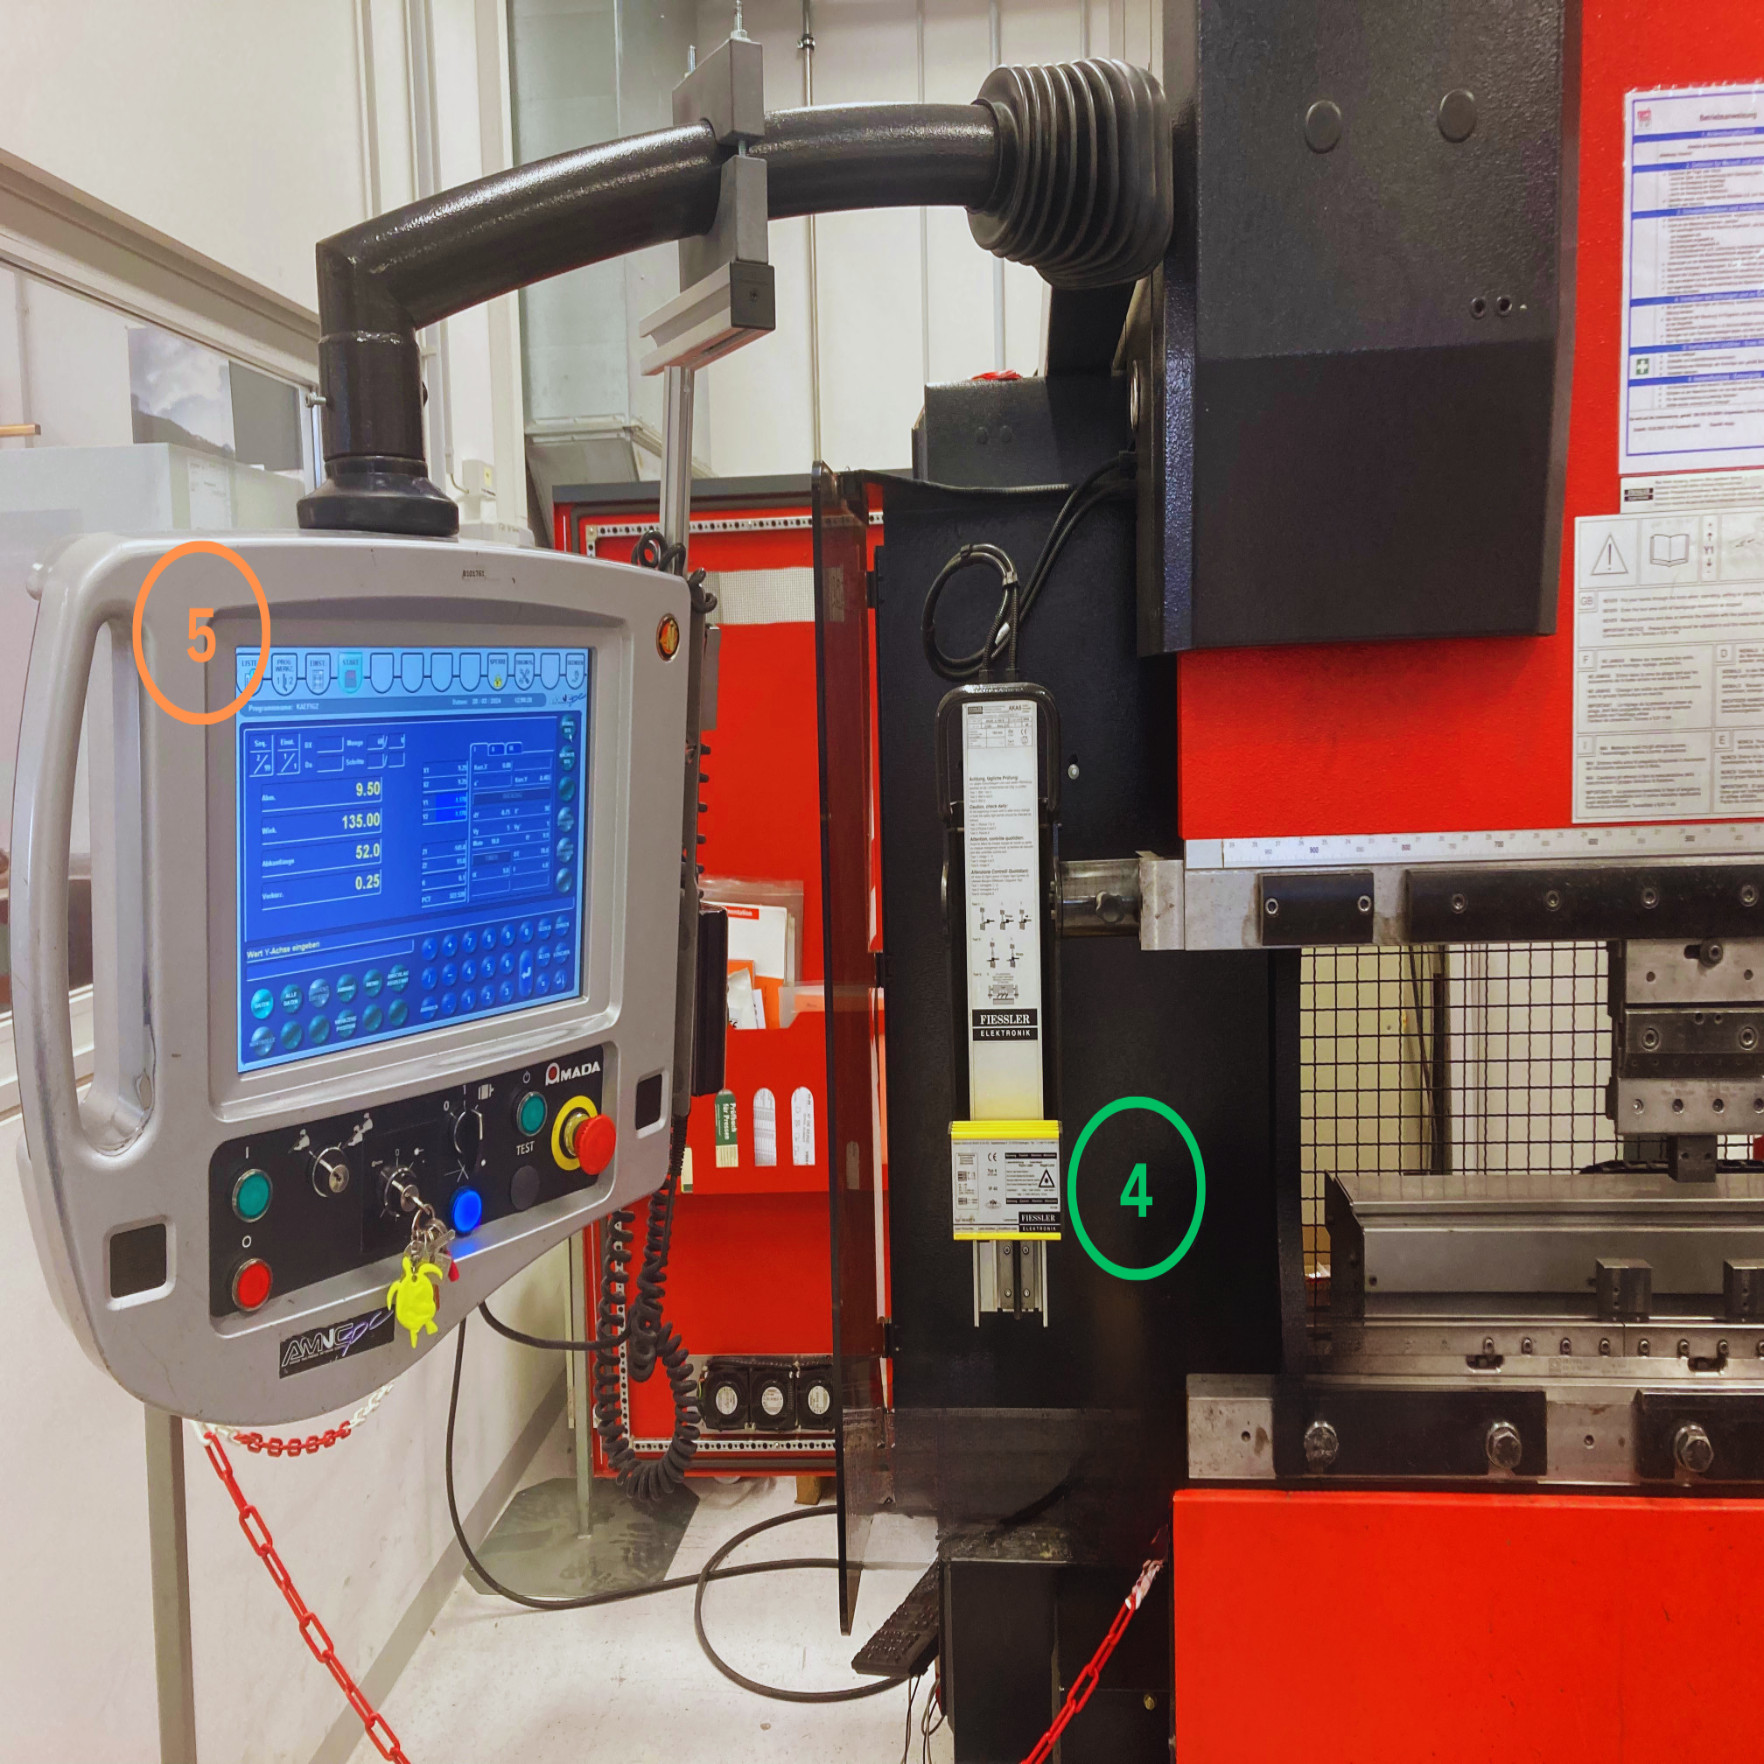
\includegraphics[width=\textwidth]{figures/bending_machine2.png} % Replace with your image file
        \label{fig:bending_machine_sub1}
    \end{subfigure}\hfill
    \begin{subfigure}{0.355\textwidth}
        \centering
        \includegraphics[width=\textwidth]{figures/bending_machine1.png} % Replace with your image file
        \label{fig:bending_machine_sub2}
    \end{subfigure}
    \caption{\hyperref[acro:AMADA]{AMADA} Bending Machine 1) Marker 2) Bending station 3) Laser height 4) Laser monitoring 5) \hyperref[acro:TFT]{TFT} Touch screen}
    \label{fig:bending_machine}
\end{figure}

\begin{table}[h!]
    \centering
    \begin{tabular}{ll}
        \MakeUppercase{\textbf{Attribute}} & \MakeUppercase{\textbf{Value}} \\
        \hline
        \textbf{Model} & HFP 50-20 \\
        \textbf{Manufacturer} & \hyperref[acro:AMADA]{AMADA} (France) \\
        \textbf{Year of manufacture} & 2005 \\
        \textbf{Drive} & Hydraulic press brake \\
        \textbf{Pressing capacity} & 500 kN \\
        \textbf{Working length} & 2090 mm \\
        \textbf{Distance between frames} & 1665 mm \\
        \textbf{\hyperref[acro:CNC]{CNC} control} & AMADA AMNC \hyperref[acro:3D]{3D}-graphic \\
        & with \hyperref[acro:TFT]{TFT} color screen \\
        \textbf{controlled axes} &  Y1/Y2; X1/X2; R1/R2; Z1/Z2 \\
        \textbf{Open height} & 470 mm \\
        \textbf{Stroke} & 200 mm \\
        \textbf{Bending Speed} & 10 mm/s \\
        \textbf{Approach Speed} & 100 mm/s \\
        \textbf{Return Speed} & 100 mm/s \\
        \textbf{Laser monitoring} & FIESSLER \\
        \textbf{Length x width x height} & 3458 mm x 2450 mm x 2450 mm \\
        \textbf{Weight} & 4850 kg \\ \hline
    \end{tabular}
    \caption{Bending Machine Specifications (Source: \cite{bmspecifications})}
    \label{tab:machine_specifications}
\end{table}

